\documentclass[a4paper,11pt]{article}
\usepackage[a4,ieis, themeblue]{tuepdfscreen2008}
\usepackage[english]{babel}
\graphicspath{{figures/}}
\usepackage{amsmath,amssymb,amsthm,mathtools,bm,etoolbox, cases, commath}
%\usepackage{mathtime} 
%\setstatustext{Stochastic Operations Research}       % This text is placed in the upper left corner of the poster and can be left empty
%\titlelogo[height=2.8cm]{eurandomlogo}               % You can use this command to insert one logo.

\titleright{\textbf{Operations, Planning, Accounting and Control Group, \\
Department of Industrial Engineering,  
Eindhoven University of Technology, 
The Netherlands
}}      % You can use this commnad INSTEAD OF the \titlelogo command
                                                              % to insert text in the upper right part of the poster (or e.g. multiple logos)


\begin{document}
\begin{slidetop}
\slidetitle[Paul Melkert]{Conditional Correlation Modeling using Machine Learning and Multivariate GARCH}
\begin{multicols}{2}
A new semiparametric multivariate volatility model is proposed, which integrates parametric univariate GARCH specifications for the conditional volatilities with nonparametric machine learning estimators for the conditional correlations. Consider a $k$-dimensional financial log return series $r_t = (r_{1,t}, \dots, r_{k,t})'$:
\begin{align} 
	r_t = H^{1/2}_t z_t, \label{eq:returns_model} \nonumber
\end{align}
where conditional variance-covariances of log returns $r_t$ is denoted by a $k\times k$ positive definite matrix $H_t$, $H_t^{1/2}$ its Cholesky decomposition, and $z_t$ denotes a $k \times 1$ vector of i.i.d. standard normal random variables. We consider a reparameterization of $H_t$, i.e. $H_{t}=D_{t}R_{t}D_{t}$, where $D_t$ is a diagonal matrix with conditional volatility of each marginal log return series on its diagonal and matrix $R_t$ includes all pairwise correlations $\rho_{i,j,t}$:

\begin{align} \label{eq:covariance_decomposition} 
	\scalebox{0.78}{
		\begin{pmatrix} h_{1,1,t}^{1/2} &&0 \\ &\ddots \\ 0 &&h_{k,k,t}^{1/2} \end{pmatrix} 
		\begin{pmatrix} 1 &\rho_{1,2,t} &\cdots &\rho_{1,k, t} \\ \rho_{2,1,t} &1 & &\rho_{2,k, t} \\ \vdots &&\ddots &\vdots \\ \rho_{k, 1,t} &\rho_{k, 2,t} &\cdots &1 \end{pmatrix} 
		\begin{pmatrix} h_{1,1,t}^{1/2} &&0 \\ &\ddots \\ 0 &&h_{k,k,t}^{1/2} \end{pmatrix}, \nonumber
		}
\end{align}
Diagonal elements of matrix $D_t$ are modeled parametrically using GARCH(1,1) and GJR-GARCH(1,1) specifications and conditional correlation matrix $R_t$ is estimated in a nonparametric manner using machine learning algorithms k-nearest neighbor (KNN) and random forest (RF) of Breiman~\cite{BR2001}. A parsimonious learner model specification, with the covariate space constructed using Pearson and Kendall sample correlations from moving windows, ensures that the model remains flexible and easy to estimate in high dimensional systems. Proposed semiparametric multivariate volatility model is applied to the 30 constituents included in the Dow Jones Industrial Average index and model adequacy is verified in terms of a common downside market risk measure Value-at-Risk (VaR):

\begin{align}
	VaR_{\alpha} = inf\{l \in \mathbb{R}:P(L>l) \le 1-\alpha\}, \nonumber
\end{align}

where $\alpha \in (0,1)$ and $F_L(l) = P(L \le l),$ denotes the distribution function of corresponding loss distribution. A failure test of unconditional coverage (Kupiec) and an independence test (Christoffersen) are considered to statistically evaluate proposed model against a parametric conditionally heteroscedastic class of models, the dynamic conditional correlation model of Engke~\cite{EN2002}, and to detect any misspecification of the risk model. It is demonstrated that proposed model is able to capture interesting conditional properties in correlations and that it shows competitive performance with the DCC model, both in tranquil market conditions (mid-1990's) and volatile market conditions (2000-2001 Dot-com bubble); the likelihood of a VaR exceedance does not depend greatly on whether a VaR exceedance occurred on the previous day. Moreover, the null hypothesis that the total number of VaR exceedances equals the expected number of VaR exceedances, given independence, is satisfied for a variety of model specifications. This can also be seen in Figure~\ref{fig:graph}, which shows the backtest results for unconditional coverage (Kupiec test).
\begin{center}
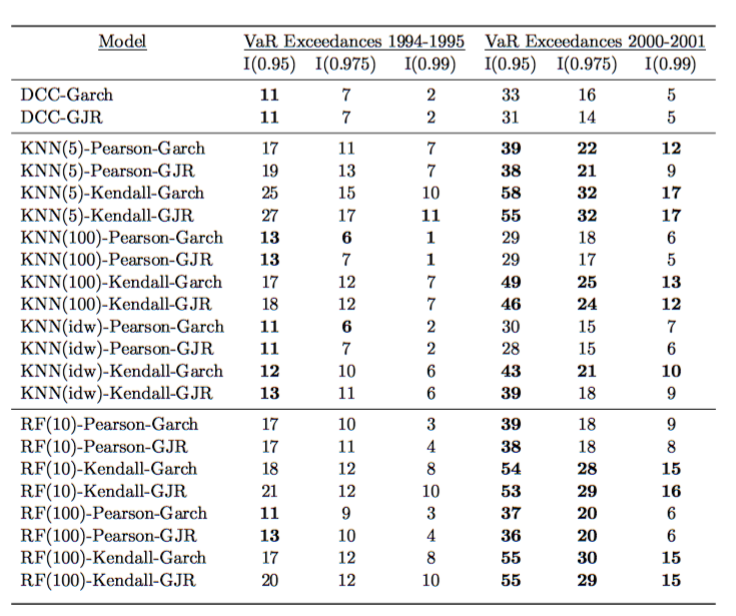
\includegraphics[scale=0.55]{kupiec_test}
\figcaption{Test results of unconditional coverage (Kupiec test) at higher quantiles of the loss distribution in tranquil and volatile market conditions. Bold face indicates rejection.\label{fig:graph}}
\end{center}

\begin{thebibliography}{99}
\bibitem{BR2001}
Leo Breiman. Random forests. Machine Learning, 45(1):5-32, 2001.
\bibitem{EN2002}
Robert Engle. Dynamic conditional correlation: A simple class of multivariate generalized autore- gressive conditional heteroskedasticity models. Journal of Business \& Economic Statistics, 20 (3):339-350, 2002.
\end{thebibliography}
\end{multicols}
\end{slidetop}

\end{document}

